\documentclass[../differential_methods.tex]{subfiles}
\begin{document}
\section{Aula 20 - 17 de Junho, 2026}
\subsection{Motivações}
\begin{itemize}
	\item Domínios de Dependência;
	\item Condição CFL;
	\item Characteristics Tracing.
\end{itemize}
\subsection{Domínio de Dependências}
A aula de hoje é particularmente importante no entendimento das equações hiperbólicas.
Começamos vendo mais um método, conhecido como \hypertarget{beam_warming}{\textbf{método beam-warming}}, que tem acurácia de ordem 2 unilateral, obtido de forma parecida ao Lax-Wendroff, mas com aproximações de \(u_x\) e \(u_{xx}\) em \(x_{j}\), começando pela mesma discretização, mas usando diferenças regressivas ao discretizar ambos. Se \(a\) for positivo,
\[
	\boxed{U_{j}^{n+1} = U_{j}^{n} - \frac{a\Delta t}{2\Delta x} (3U_{j}^{n} - 4U_{j-1}^{n} + U_{j-2}^{n}) + \frac{a^{2}\Delta t^{2}}{2\Delta x^{2}}(U_{j}^{n}-2U_{j-1}^{n} + U_{j-2}^{n})}
\]
\begin{exr}
	Deduza o método beam-warming e mostre que ele será estável se \(0 < \nu \leq 2\); deduza o mesmo para o caso \(a < 0\), mas para \(-2 \leq \nu < 0 \).
\end{exr}
\begin{exr}
	Faça as análises de Von-Neumann dos métodos da aula passada e do beam-warming.
\end{exr}

Para o próximo raciocínio, vamos utilizar como base o \hyperlink{up_wind}{\textit{método upwind}} discretizado; tomando um ponto \(u(x_{j}, t_{n})\approx U_{j}^{n}\), queremos que a solução aproxime \(u(x_{j}, t_{n})\), e por ser um problema hiperbólica, a informação para isso vem da curva característica que carrega a informação para o ponto desejado, que tem forma
\[
	u(x_{j}, n\Delta t) = \eta (x_{j}-a t_{n}),
\]
tal que a solução exata depende apenas do ponto \(x_{j}-at_{n}\). Logo, fazendo mudanças na condição inicial em qualquer ponto diferente dele \textbf{não irá alterar a solução!}; essa é a direção da nossa análise de hoje, o chamado \textbf{domínio de dependência da solução exata}: \(\mathcal{D}_{E}(u(x, t)),\)
que, neste caso, é \(\mathcal{D}_{E}(u(x, t)) = \{x-at\}\), o que significa que, se queremos calcular a solução exata em qualquer ponto, ela dependerá apenas dos pontos no domínio de dependência. Assim, a definição é:
\begin{def*}
	O \textbf{domínio de dependência real} de uma solução exata para uma EDP é o conjunto de todos os pontos iniciais que afetam o valor da solução do método em um ponto \((x, t)\). Por outro lado, o \textbf{domínio de dependência numérico}, \(\mathcal{D}_{N}\), é o conjunto de pontos da malha inicial ou de passos anteriores que afetam o valor aproximado pelo método numérico em \((x_{j}, t_{n})\) \(\square\)
\end{def*}
Se fizermos um refinamento de malha (em \(\Delta t\) e em \(\Delta x\)) e recalcularmos o domínio de dependência, nota-se que ele passa a ficar mais refinado, até que, no limite ao infinito, torna-se um intervalo em torno dos pontos na fronteira (?).
Para sistemas hiperbólicos, é possível mostrar que
\[
	\mathcal{D}_{N}(U_{j}^{n}) = \{x_{j}-\lambda_p T:\; p = 1, \dotsc , s\}.
\]

Queremos convergência do método numérico; nessa situação da malha com o domínio de dependência, o método converge quando \(\Delta t\) e \(\Delta x\) vão para zero? Não! O motivo é que, pela forma que o método foi construído, as curvas características e as escolhas de \(\Delta t\) e \(\Delta x\) continuam pegando informação de um ponto fora do domínio de dependência da solução real, então o método nunca enxerga os pontos onde estão as soluções reais.
Caso as características estivessem dentro do domínio do método, aí sim a convergência iria depender de estabilidade e consistência, mas se ele já falha em ter as características no domínio numérico, o método já falha:
\hypertarget{cfl_condition}{\begin{theorem*}[Condição Courant-Friedrichs-Lewy (CFL)]
		Um método numérico só pode ser convergente se seu domínio de dependência numérico contém o domínio de dependência real da EDP, pelo menos nos limites \(\Delta t\) e \(\Delta x\) indo a 0.
	\end{theorem*}}
Para consertar um problema de domínio de dependência separados, é preciso ajustar a malha, para obter um estêncil que inclua os dois.

Para o método upwind, o domínio de dependência real e numérico para um ponto \((x_{j}, t_{n})\) são, respectivamente,
\[
	\mathcal{D}_{E}(u(x_{j}, t_{n})) = \{x_{j}-at_{n}\} \quad\&\quad \mathcal{D}_{N}(U_{j}^{n}) = [x_{j}-n\Delta t, x_{j}],
\]
tal que a \hyperlink{cfl_condition}{\textit{Condição CFL}} passa a ser
\[
	\mathcal{D}_{E}\subseteq \mathcal{D}_{N} \Longleftrightarrow x_{j}-nh \leq x_{j}-an\Delta t\leq x_{j} \Longleftrightarrow -n\Delta x \leq -a_{n}\Delta t\leq 0,
\]
que resulta na condição
\[
	\frac{a\Delta t}{\Delta x}\leq 1.
\]
Parece familiar? Deveria, pois é a condição de estabilidade para o método upwind; no entanto, nem todo caso vai ser assim: a condição CFL é uma condição \textit{necessária}, mas não suficiente (um ``somente se'' do se, e somente se), e a condição de estabilidade caracteriza a estabilidade, que é parte da convergência.
Portanto, a \textbf{condição CFL NÃO É uma condição de estabilidade!!} Eles até vão coincidir para esses casos lineares e simples, mas nada garante quando saímos deles.

\begin{example}[Lax-Wendroff]
	Como o \hyperlink{lax_wendroff}{\textit{Lax-Wendroff}} tem um esquema centrado, o domínio de dependência dele forma uma pirâmide:
	\[
		\mathcal{D}(x_{j}, t_{2}) = \{x_{j-2}, x_{j-1}, x_{j}, x_{j+1}, x_{j+2}\}
	\]
	em \(n=2\) e
	\[
		\mathcal{D}(x_{j}, t_{4}) = \{x_{j-4}, \dotsc , x_{j}, \dotsc , x_{j+4}\}
	\]
	para \(n=4\).
	\begin{figure}[H]
		\begin{center}
			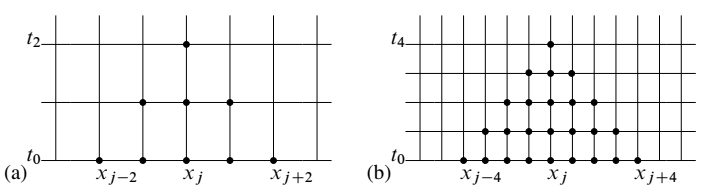
\includegraphics[height=\textheight, width=\textwidth, keepaspectratio]{./Images/lax_wendroff_18.png}
		\end{center}
	\end{figure}
\end{example}
\begin{example}[Beam-warming]
	No \hyperlink{beam_warming}{\textit{Beam-warming}}, como a cada \(\Delta t\) que é percorrido, \(2\Delta x\) são também, o domínio de dependência real estar dentro do numérico dele é justamente que \(0>\nu \geq 2\) (ou sinais invertidos), e a condição a estabilidade dele requer que o número de Courant seja menor ou igual a 2.
\end{example}

\begin{tcolorbox}[
		skin=enhanced,
		title=Observação,
		fonttitle=\bfseries,
		colframe=black,
		colbacktitle=cyan!75!white,
		colback=cyan!15,
		colbacklower=black,
		coltitle=black,
		drop fuzzy shadow,
		%drop large lifted shadow
	]

	Com o método central que começamos essa seção, ele ilustra um caso onde a \hyperlink{cfl_condition}{\textit{condição CLF}} é satisfeita, mas mesmo assim não converge -- para ele, a condição CFL é \(| a |\frac{\Delta t}{\Delta x}\leq 1\), que é satisfeita.
\end{tcolorbox}

\subsection{Acompanhamento de Características e Interpolação}
Vamos dar uma olhada no chamado Acompanhamento de características (\textit{characteristic tracing}), considerando o caso \(u(x_{j}, t_{n+1})\) e que \(a \frac{\Delta t}{\Delta x} \leq 1\). Traçar as características de forma retrograda no tempo dentro da malha \(x_{j}\) resulta, para cumprir a \hyperlink{cfl_condition}{\textit{condição CFL}}, na relação
\[
	u(x_{j}, t_{n+1}) = u(x_{j}-a\Delta t, t_{n}), \quad x_{j-1} < x_{j}-a\Delta t < x_{j},
\]
que é representado pela imagem
\begin{figure}[H]
	\begin{center}
		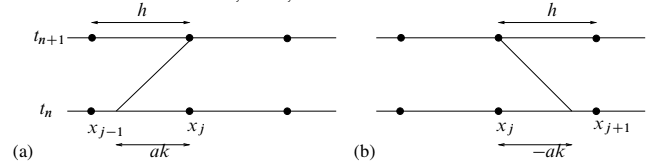
\includegraphics[height=\textheight, width=\textwidth, keepaspectratio]{./Images/characteristics_Interpolation_20.png}
	\end{center}
\end{figure}
Como já sabemos a solução no ponto \(U_{j-1}^{n}\) e em \(U_{j}^{n},\) podemos usar um polinômio interpolador para encontrar ela em \(U_{j}^{n+1}\); é necessário um polinômio interpolador avaliado em \(x_{j}\) que resulte em um termo com \(j-1\):
\[
	p(x) = (x-x_{j-1})U_{j}^{n} + (x_{j}-x)U_{j-1}^{n}
\]
Para os termos multiplicando as aproximações ficarem de acordo com as aproximações, precisamos dividir ambos por \(\Delta x\), resultando em
\[
	p(x) = \frac{x-x_{j-1}}{\Delta x} U_{j}^{n} + \frac{x_{j}-x}{\Delta x}U_{j-1}^{n},
\]
e quando x for \(x_{j}\) ou \(x_{j-1}\), apenas um deles irá restar. Este processo é chamado de \textbf{interpolação de características}, e aplicando ele ao valor inicial \(x_{j}-a\Delta t\), segue que
\[
	U_{j}^{n+1}=p(x_{j}-a\Delta t) = U_{j}^{n} + ((x_{j}-a)-x_{j})\biggl(\frac{U_{j}^{n}-U_{j-1}^{n}}{\Delta x}\biggr) = U_{j}^{n}-\frac{a\Delta t}{\Delta x}(U_{j}^{n}-U_{j-1}^{n}),
\]
tal que a interpolação linear feita entre \(U_{j-1}^{n}\) e \(U_{j}^{n}\) resultou no \hyperlink{up_wind}{\textit{método upwind}}! Aproveitamos a informação sobre propagação de informação de características e tentamos aproveitar ela, resultando num dos método que havíamos visto antes, mas por outro caminho, dando outra fábrica de métodos para usarmos.

O mesmo processo pode ser usado para obter o \hyperlink{lax_wendroff}{\textit{Método de Lax-Wendroff}} e \hyperlink{beam_warming}{\textit{Beam-warming}}, com o primeiro usando uma interpolação quadrática entre \(U_{j-1}^{n},\; U_{j}^{n}\) e \(U_{j+1}^{n}\), enquanto o segundo usa uma interpolação quadrática de \(U_{j-2}^{n},\; U_{j-1}^{n}\) e \(U_{j}^{n}\).
\begin{exr}
	Deduza os dois métodos mencionado usando interpolação de características. Deduza, também, o método resultante do polinômio interpolador linear que usa \(U_{j-1}^{n}\) e \(U_{j+1}^{n}\).
\end{exr}

Alguns comentários a parte que valem a pena (talvez apenas 1, dependendo do quanto eu entender) fazer incluem o problema de Riemann, que afeta principalmente os métodos advecção-difusão, pois é caracterizado por uma condição inicial em salto, e a descontinuidade resulta em difusão extrema, que foram os que sobraram pra lidar com dados iniciais com grande variação!
O que resta, portanto, é construir métodos melhores, mas construídos de maneira mais sofisticada, principalmente para os casos não lineares -- eles introduzem um problema completamente novo e à parte. Por exemplo, uma equação usada bastante nesse tipo de problema é
\[
	u_t + u u_x = 0,
\]
que parece até que simples, mas mesmo que fosse dada uma condição inicial suave, como as características têm inclinação dada pela recíproca da velocidade de transporte, a u em si explode para infinito rapidamente quando chega ao fim da inclinação suave! A solução fica cada vez menos suave, até chegar ao ponto de ficar descontínua, resultando também em cruzamento de características -- duas características chegam ao mesmo ponto e torna-se impossível distinguir qual das soluções é a certa.
Logo, mesmo com condições iniciais suaves, os problemas lineares ainda ficam descontínuo, e o que significa uma solução descontínua de uma equação que tem derivadas?

Por conta disso, entram os métodos de volumes finitos ou elementos finitos, porque os métodos de diferenças finitas não dão conta desses grandes problemas.

\begin{tcolorbox}[
		skin=enhanced,
		title=Lembrete!,
		after title={\hfill Interpolação},
		fonttitle=\bfseries,
		sharp corners=downhill,
		colframe=black,
		colbacktitle=yellow!75!white,
		colback=yellow!30,
		colbacklower=black,
		coltitle=black,
		%drop fuzzy shadow,
		drop large lifted shadow
	]
	O \textbf{polinômio interpolador} é o polinômio de menor grau possível (logo, é único a menos de coeficiente líder) que passe por todos os pontos de um estêncil; em particular, um polinômio
	\[
		p(x) = a_{0}+ a_1x + \dotsc +a_{n}x^{n}
	\]
	\textbf{interpola} os dados se \(p(x_{j}) = y_{j}\) para todo j entre 0 e n, com os dados sendo \((x_{0}, y_{0}), \dotsc , (x_n, y_{n})\).

	A \textbf{interpolação de Lagrange} tem forma
	\[
		p(x) = \sum\limits_{i=0}^{n}\frac{p(x)}{p'(x_{i})(x-x_{i})}y_{i},
	\]
	e a \textbf{interpolação de Newton} entre um polinômio \(p_{n}\) de grau até n interpolado com um função f em pontos \(x_{i},\; i=0, 1, \dotsc , n\) é dada por
	\[
		p_{n+1}(x) = p_{n}(x) + a_{n+1} \prod\limits_{i=0}^{n}(x-x_{i}),
	\]
	onde, usando a notação \(w_{n}(x)\coloneqq \prod\limits_{i=0}^{n}(x-x_{i})\) para a chamada \textbf{base de Newton}, o termo \(a_{n+1}\) tem forma
	\[
		a_{n+1}\coloneqq \frac{f(x_{n+1}) - p_{n}(x_{n+1})}{w_{n}(x_{n+1})},
	\]
\end{tcolorbox}
\end{document}
